\documentclass[conference]{IEEEtran}
\usepackage{multirow}
\usepackage{color}
\usepackage{graphics}
\usepackage{rotating}
\usepackage{graphics}
\usepackage{colortbl}
\usepackage{picture}
\usepackage{algorithm}
\usepackage{algorithmicx}
\usepackage{algpseudocode}


\begin{document}
\title{CSC791 Spatial-Temporal Data Mining Project Report}
\author{Wei Fu, George Matthew, Qiang Zhang} 

\maketitle
\begin{abstract}
  Crater detection has been one fundamental task in planetary science, which has drawn great attention from fields of data mining and image processing. In this project,  typical spatial data mining algorithms for crater detection are discussed, implemented and analyzed. Based on the results of different algorithms, potential improvements are proposed.
\end{abstract}
\section{Introduction}
Craters are key structures formed by the collisions of meteorioids, asteroid or comet with planetary surface. To investigate past and future geological informaiton, craters detection methods or tools with high precision are demanded. Manual inspection of images is one mainly used method. However, due to the increasing huge amount of craters needed to be identified in very high resolution planetary images, this widely used method seems out-dated but automatic detection is the only practical solution to such tasks. Several reasons \cite{kim2005automated} can explain this:
\begin{itemize}
 \item The lighting conditions result in different qualities of the images, which would affect the detecting accuracy.
 \item Some geographical features, like volcanos, have similar morphological characteristics as craters.
 \item Crater rims are frequently eroded due their formation millions of years ago. 
\end{itemize}

In this project, we're trying to learn and implement algorithms that address all these issues. 
We choose \cite{ding2011subkilometer} as a main reference to build a robust and practical crater detection framework. Based on this, a new detection algorithm will be designed to further improve the performance .

\section{Problem definition}
The automatic detection algorithms should solve the above challenges. Specifically, two problems are to address: (1) based on the candidates of craters, how to classify them accurately into crater and non-crater classes? (2) given a training dataset including crater and non-crater examples, how to make the algorithm applicable to detect the craters in other data sets.
\section{State-of-the-art}

Salamuniccar\cite{salamuniccar2008open} provided an extensive review of previous work on crater detection algorithms, which can be divided into two categories: supervised and unsupervised-learning methods. 

The unsupervised approcahes identify crater rims in an image as circular or elliptical features\cite{bandeira2007impact,cheng2003optical,honda2002mining,leroy2001crater,galloway2014image}. All of the methods fall in this category would use Hough Transform or similar image processing methods to improve the performance of crater edge detection Specifically, in \cite{leroy2001crater}, a new robust method is proposed to infer curvature estimation from noisy space data  to compute a dense saliency map corresponding to the position and shape of the craters. The detected craters in the image are matched with the craters projected from a 3D model. Authors of \cite{bandeira2007impact} presented a methodology that brought number of techniques in the fields of image processing and pattern recognition, including candidate selection, template matching and final identification based on the probability to detect impact craters on images. Rie et al.\cite{honda2002mining} proposed to group original images according to spatial frequency patterns and both optimized parameters setts and noise reduction techniques used to identify candidate craters and false candidates are excluded using a self-organizing map approach.

Supervised methods are designed based on data mining techniques, where algorithms use the labeled data sets to train a learner and then identify craters on new data sets with this learner. Jinhao et al. \cite{Jihao2015selected} proposed to generate Gist feature from selected training samples and the crater detection is conducted using Gist feature vectors with random forests classification. Siyi et al.\cite{siyi2011image} used semi-supervised Active Class Selection algorithm to iteratively enrich an original small training set, without additional human labeling effort, to detect craters form a large volume of images. Ying et al. \cite{ying2013crater} proposed to integrate the Least Absolute Shrinkage and Selection Operator method  with Bayesian network classifier for this task. The work we mainly referred designed a framework, which used a supervised boosting learning algorithms and transfer learning methods to classify crater candidates based on the texture features extracted from the original images.


\section{Algorithms}
In this projects, we implemented tree algorithms, including Boost algorithm, Naive algorithm and Transfer Learning algorithm, proposed in \cite{ding2011subkilometer}.
\begin{figure}[!h]
\begin{center}
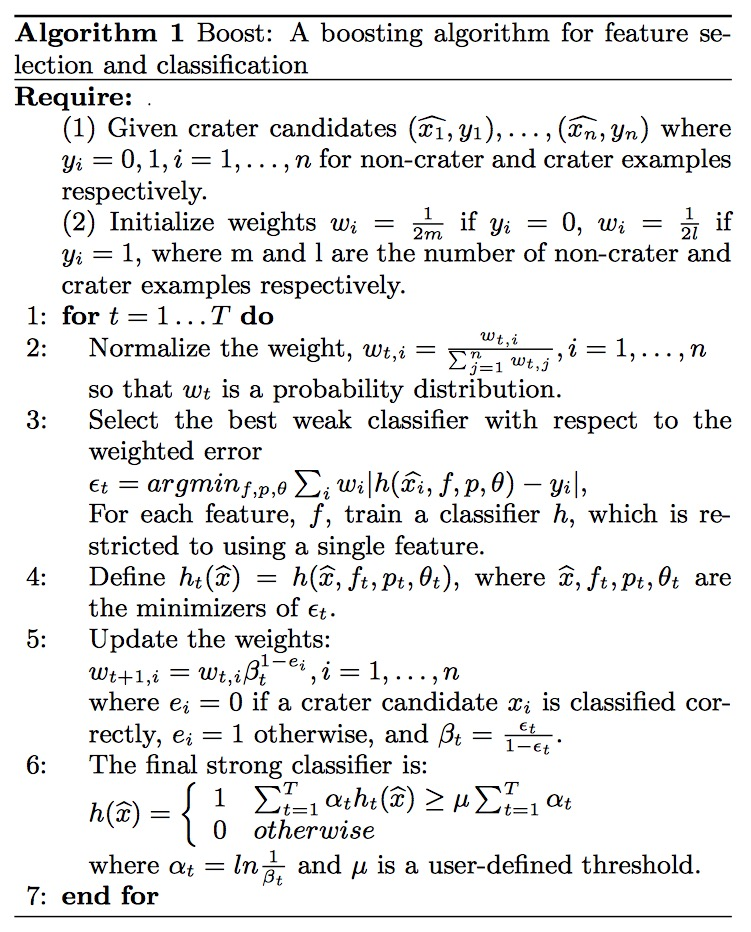
\includegraphics[scale=0.34]{boost.png}
\label{default}
\end{center}
\end{figure}

\begin{figure}[!htb]
\begin{center}
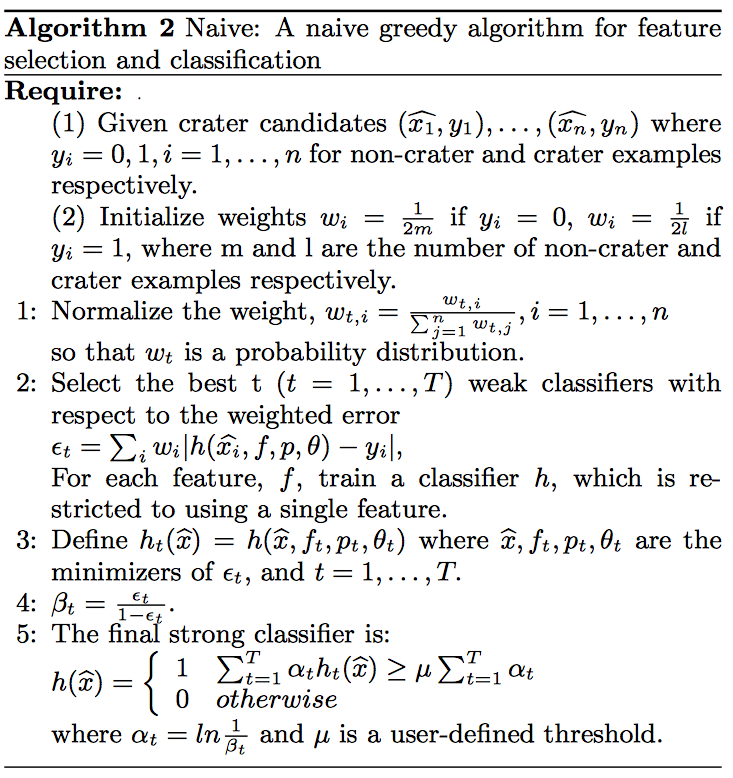
\includegraphics[scale=0.34]{naive.png}
\label{default}
\end{center}
\end{figure}
The Boost algorithm generates a sequence of weak classifers $h_t(f)$ and combine them through a weighted approach to build a strong classifier $H(\hat{x})$:
\begin{equation}
 H(\hat{x}) = \sum_{t=1}^{T}\alpha_th_t{f}
\end{equation},
where T is the number of iterations, $t = 1,...,T$, $\hat{x} = <f_1,...,f_N>$ is the feature vector that describes a crater candidate; $f \in {f_1,...,f_N}$ is the single feature used to construct a weak classifier $h_t(f)$ and $\alpha_t$ is the weight of hypothesis $h_t(f)$. The Boost algorithm iteratively selects one feature at a time and stops when reaching T iterations; each iteration the Boost algorithm will choose a best feature, which includes weak classifier learning , features selection and weight updating. More details are described in algorithm 1.


The Naive algorithm is to reduce the time complexity required by Boost algorithm. This algorithm uses the same weak classifier learning step and selects the top T best features using the weighted error sum in the step of feature selection as a criterion without any further iterations on weight updating.

The Transfer Learning algorithm has the same three steps as Boosting algorithm, but the weight updating step is different. In Boosting algorithm, both training and testing data sets are drawn independently and identically from an underlying distribution and it is not expected to perform well if the testing data has a different distribution from the training data. The method used here is to build the  strong classifier sequentially. Details are presented in {\it weight updating}step in Algorithm 3.

\begin{figure}[!hb]
\begin{center}
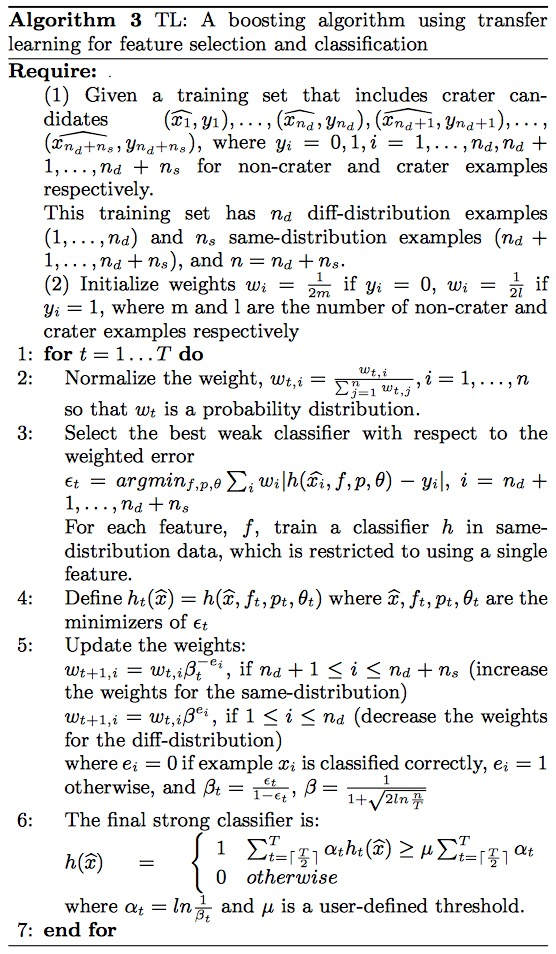
\includegraphics[scale=0.45]{TL.png}
\label{default}
\end{center}
\end{figure}


\begin{figure*}[ht]
\begin{center}
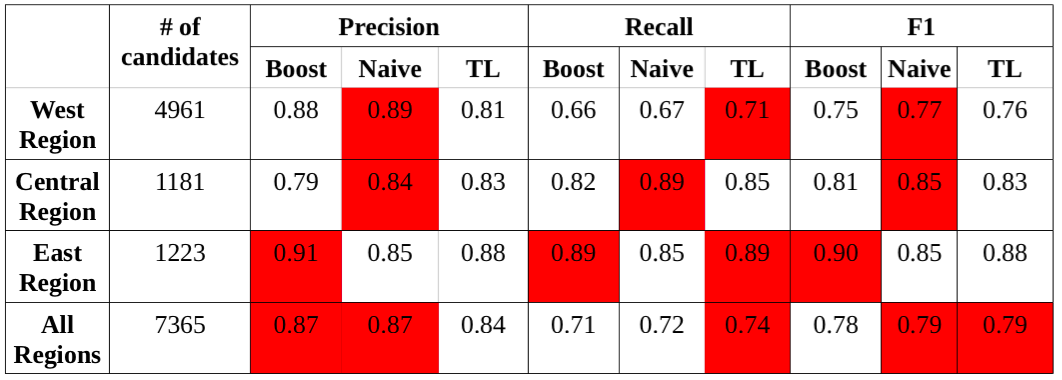
\includegraphics[scale=0.45]{T_50.png}
\caption{Performance of Boost, Naive, and TL algorithms;T= 50; Boost : mu =0.475; ForGreedy: mu = 0.325; Transfer: mu = 0.5.}
\label{T50}
\end{center}
\end{figure*}

\begin{figure*}[ht]
\begin{center}
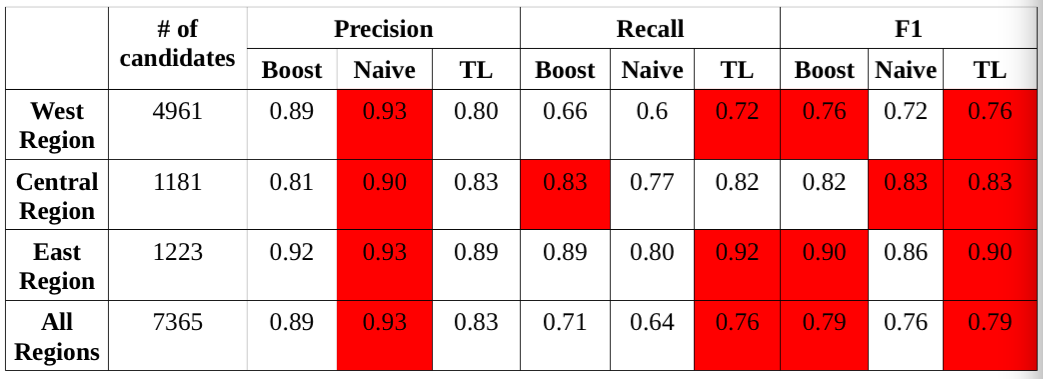
\includegraphics[scale=0.45]{T_150.png}
\caption{Performance of Boost, Naive, and TL algorithms;T= 150; Boost : mu =0.475; ForGreedy: mu = 0.325; Transfer: mu = 0.5.}
\label{T150}
\end{center}
\end{figure*}
\subsection{Dataset description}
\section{Experimental results}

The dataset used in this project is from the same source as \cite{ding2011subkilometer}, which is a portion of the Hight Resolution Stereo Camera nadir panchromatic image h0905. The selected image has the resolution of 12.5 meters/pixel and the size of 3,000 by 4,500 pixels. The image is divided into west region, central region and east region, which include $4961$,$1181$ and $1223$ crater candidates, respectively. For some unknown reason,this is different from the numbers in \cite{ding2011subkilometer} even though we got this data set from their website.
\subsection{Analysis}
The results  generated by our implementation is listed in Fig.\ref{T50} and Fig. \ref{T150}. We can see that the best precision is produced by the naive algorithm, the best recall is produced by the transfer learning algorithm and the best F1 score is predicted by the transfer learning algorithm. We can also see that the recall of the naive algorithm reduces when we increase the number of features but the transfer learning algorithm improves when we use more features. The results shown here are different from \cite{ding2011subkilometer} in terms of ranks of these three algorithms for different goals. One possible reason is that the dataset we used offered by Dr.Ding is different from the ones they used in the paper.

\section{Summary}
In the first phase of our projects, we  did literature review, found related data sets and implemented three algorithms in the target paper. The results we got are different from the original paper. We would verify our results by another version of implementation.  In next phase, we plan to implement new algorithm to improve the detection performance.
 

\bibliographystyle{unsrt}
\bibliography{CratersDetection}

\end{document}
